\section{Resultados}

\subsection{Modulação AM-DSB-SC (Double Sideband Suppressed Carrier)}

Na modulação AM-DSB-SC, espera-se observar o espectro da mensagem deslocado para as frequências laterais em torno da frequência da portadora, conforme ilustrado na Figura~\ref{fig:sinais_freq_am_dsb}. Como pode ser visualizado, a mensagem original, que é uma senoide de 1~kHz, aparece como dois impulsos simétricos em torno da portadora de 5~kHz, definida pelo QT GUI Range. Isso ocorre devido à propriedade da modulação, que desloca o espectro da mensagem para as frequências $f_c + f_m$ e $f_c - f_m$, onde $f_c$ é a frequência da portadora e $f_m$ a frequência da mensagem.

\begin{figure}[!htpb]
    \centering
    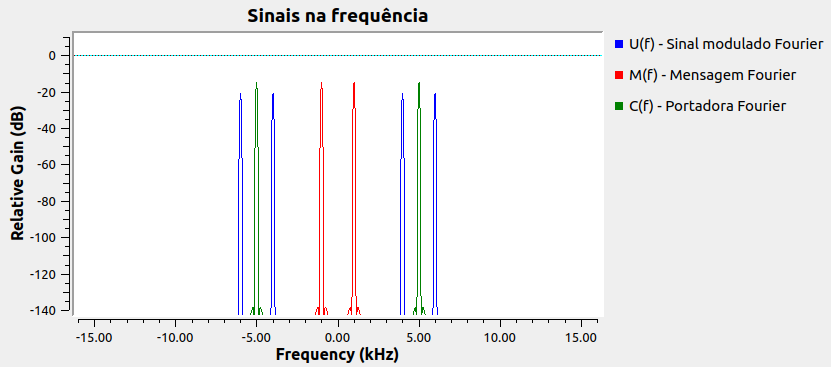
\includegraphics[width=0.4\textwidth]{images/sinais_freqe_gnu.png}
    \caption{Sinais no domínio da frequência. Fonte: Autor.}
    \label{fig:sinais_freq_am_dsb}
\end{figure}

\begin{figure}[!htpb]
    \centering
    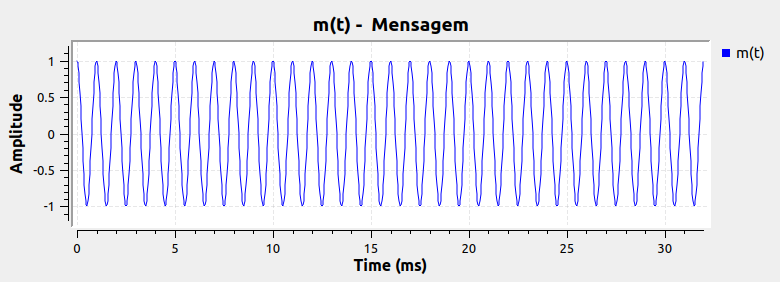
\includegraphics[width=0.5\textwidth]{images/mensagem_dsb.png}
    \caption{Mensagem no tempo. Fonte: Autor.}
    \label{fig:mensagem_tempo_am_dsb}
\end{figure}

\begin{figure}[h]
    \centering
    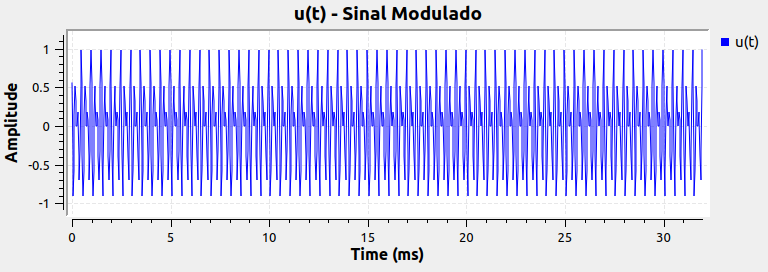
\includegraphics[width=0.4\textwidth]{images/mensagem_modulada_gnu.png}
    \caption{Mensagem modulada DSB-SC. Fonte: Autor.}
    \label{fig:mensagem_modulada_am_dsb}
\end{figure}

\subsection{Demodulação AM-DSB-SC (Double Sideband Suppressed Carrier)}

Os resultados da demodulação também estão de acordo com o esperado. Ao utilizar um filtro passa-baixa com frequência de corte superior à largura de banda da mensagem para filtrar as componentes de alta frequência geradas pela multiplicação do oscilador local, é possível recuperar o sinal original. A Figura~\ref{fig:demodulacao_am_dsb} mostra o espectro do sinal após a demodulação, evidenciando a recuperação da senoide de 1~kHz.

\begin{figure}[!htpb]
    \centering
    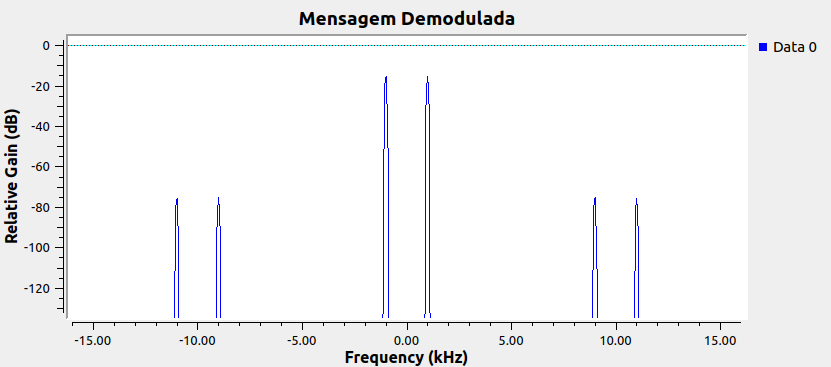
\includegraphics[width=0.4\textwidth]{images/demodulacao_am_dsb_freq.png}
    \caption{Demodulação do sinal AM-DSB-SC. Fonte: Autor.}
    \label{fig:demodulacao_am_dsb}
\end{figure}

\begin{figure}[!htpb]
    \centering
    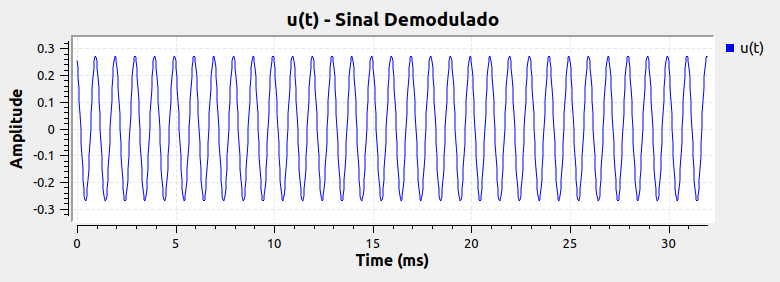
\includegraphics[width=0.4\textwidth]{images/mensagem_demodulada.png}
    \caption{Mensagem no tempo após demodulação. Fonte: Autor.}
    \label{fig:mensagem_demodulada_am_dsb}
\end{figure}

\subsection{Falta de Sincronismo e Fase de 90 Graus}
Para demonstrar que a demodulação AM-DSB-SC exige sincronismo de fase entre a portadora do transmissor e o oscilador local do receptor, a fase da portadora foi alterada para $\pi/2$, evidenciando a perda de informação no espectro. Em seguida, a frequência da portadora foi modificada para 10~kHz, mostrando a necessidade de sincronismo entre os osciladores. A Figura \ref{fig:falta_sincronismo_dsb} mostra a primeira situação quando deslocamos a fase do oscilador local para $\pi/2$, a mensagem é praticamente perdida.

\begin{figure}[!htpb]
    \centering
    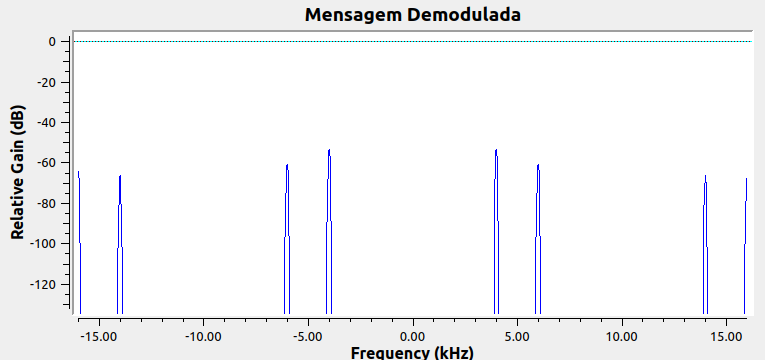
\includegraphics[width=0.4\textwidth]{images/falta_sincronismo_dsb.png}
    \caption{Espectro da mensagem quando não há de sincronismo de fase. Fonte: Autor.}
    \label{fig:falta_sincronismo_dsb}
\end{figure}

Também temos a perda da informação quando não há o sincronismo de frequência entre a portadora e o oscilador local Figura \ref{fig:sinal_sem_sincronismo_dsb}.

\begin{figure}[!htpb]
    \centering
    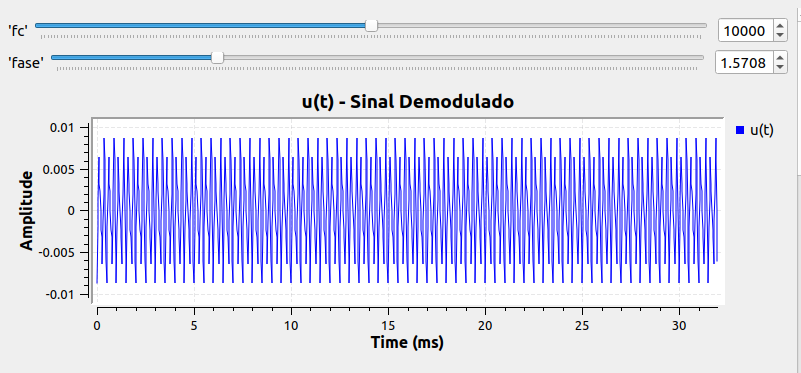
\includegraphics[width=0.4\textwidth]{images/sinal_sem_sincronismo_dsb.png}
    \caption{Sinal demodulado sem sincronismo de frequência e fase. Fonte: Autor.}
    \label{fig:sinal_sem_sincronismo_dsb}
\end{figure}

Quando temos uma fase diferente de $90^\circ$, o sinal da mensagem fica distorcido Figura \ref{fig:distorcao_dsb}, mesmo que a frequência da portadora seja igual.

\begin{figure}[!htpb]
    \centering
    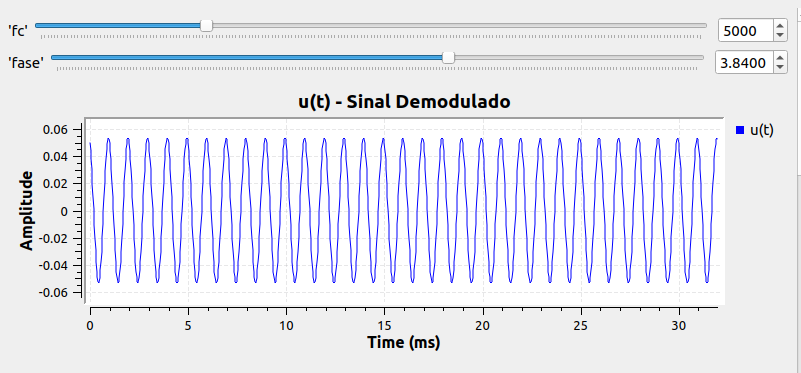
\includegraphics[width=0.4\textwidth]{images/distorcao_dsb.png}
    \caption{Distorção do sinal quando a frequência é igual à da portadora, mas a fase é diferente de 90 graus. Fonte: Autor.}
    \label{fig:distorcao_dsb}
\end{figure}

\subsection{Modulação AM}

A mensagem enviada corresponde a um cosseno de frequência 1~kHz. Foi colocado uma fase de 90 graus na portadora para envidenciar também que não é necessario sincronismo de fase. 

\begin{figure}[!htpb]
    \centering
    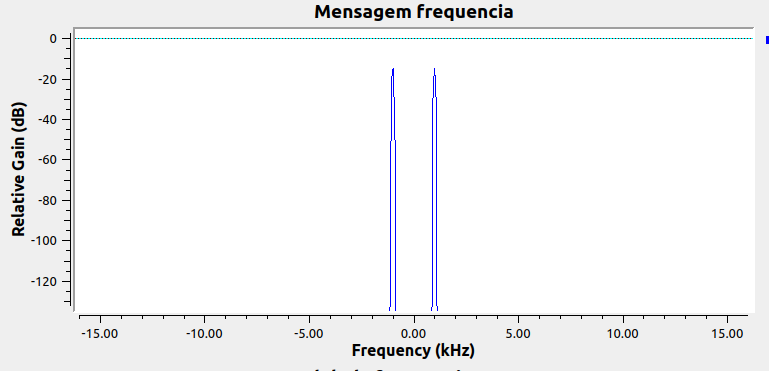
\includegraphics[width=0.4\textwidth]{images/mensagem_am_gnu.png}
    \caption{Mensagem transmitida no tempo. Fonte: Autor.}
    \label{fig:mensagem_am_tempo}
\end{figure}

O sinal modulado apresenta uma envoltória correspondente à mensagem, como esperado para modulação AM.

\begin{figure}[!htpb]
    \centering
    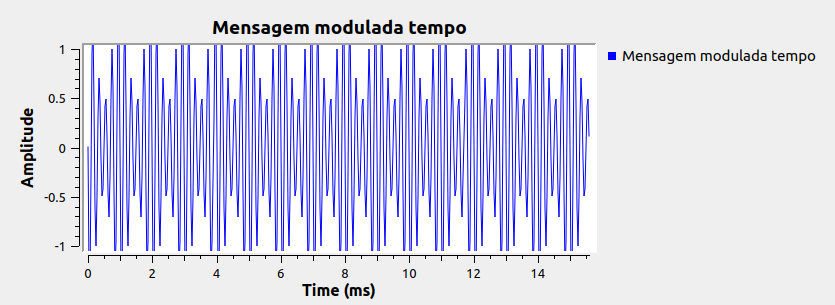
\includegraphics[width=0.4\textwidth]{images/envoltoria_gnu.png}
    \caption{Sinal AM modulado no tempo, mostrando a envoltória. Fonte: Autor.}
    \label{fig:envoltoria_am}
\end{figure}

No domínio da frequência, observa-se um componente em $f_c$ devido à portadora, além das bandas laterais em torno de $f_c$ correspondentes à mensagem.

\begin{figure}[!htpb]
    \centering
    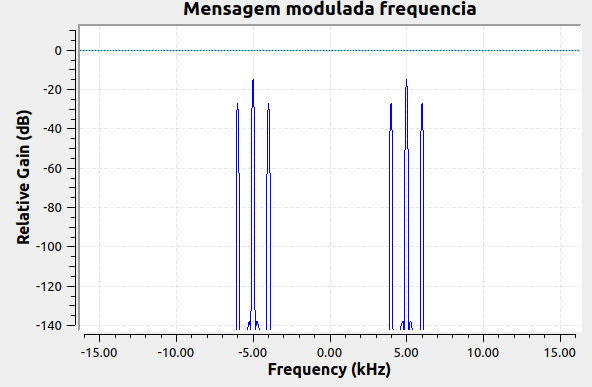
\includegraphics[width=0.4\textwidth]{images/mensagem_am_modulada_gnu.png}
    \caption{Espectro do sinal AM modulado. Fonte: Autor.}
    \label{fig:espectro_am_modulada}
\end{figure}

\subsection{Demodulação AM}

A demodulação é realizada inicialmente pela retificação do sinal, obtendo-se um sinal retificado de meia onda.

\begin{figure}[!htpb]
    \centering
    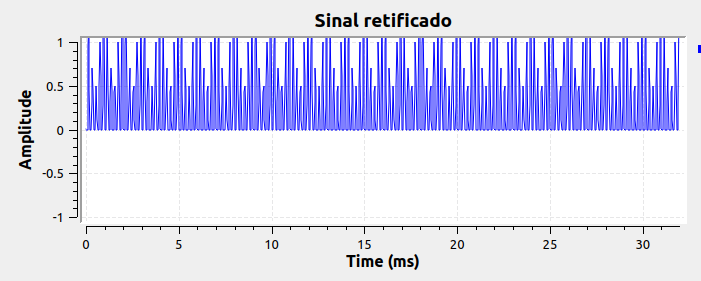
\includegraphics[width=0.4\textwidth]{images/retificado_gnu.png}
    \caption{Sinal retificado de meia onda. Fonte: Autor.}
    \label{fig:retificado_am}
\end{figure}

Após a filtragem passa-baixa e remoção da componente DC, o espectro do sinal recuperado se assemelha ao da mensagem original.

\begin{figure}[!htpbh]
    \centering
    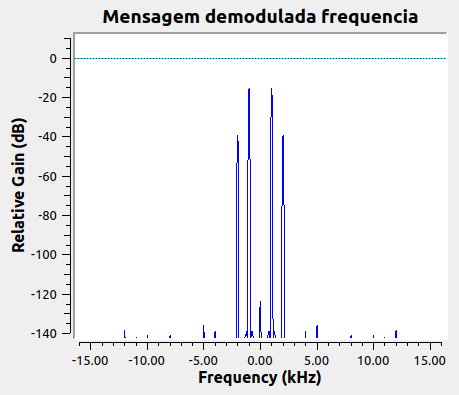
\includegraphics[width=0.4\textwidth]{images/mensagem_demodulada_gnu_espectro.png}
    \caption{Espectro do sinal demodulado. Fonte: Autor.}
    \label{fig:espectro_demodulada_am}
\end{figure}

A mensagem recuperada pode ser observada no domínio do tempo.

\begin{figure}[!htpb]
    \centering
    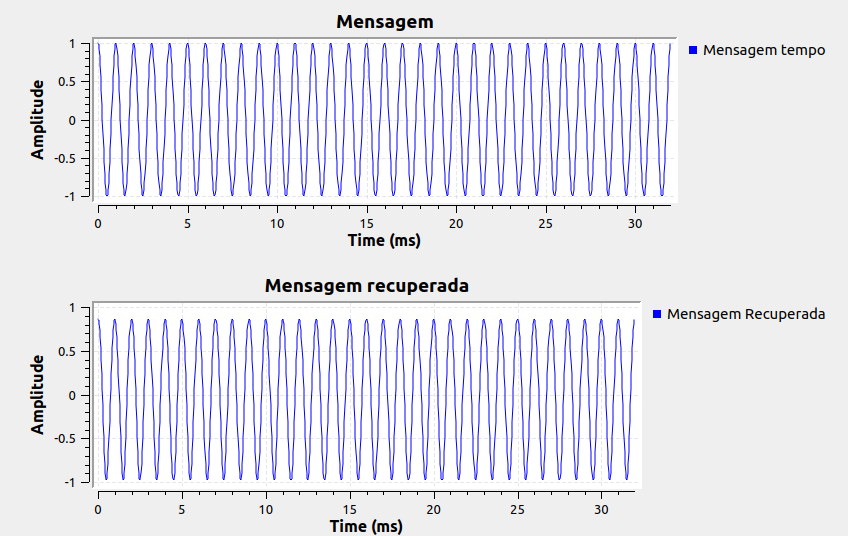
\includegraphics[width=0.4\textwidth]{images/mesagem_enviada_recuperada_am.png}
    \caption{Mensagem recuperada no tempo após demodulação. Fonte: Autor.}
    \label{fig:mensagem_recuperada_am}
\end{figure}

\subsection{Falta de Sincronismo em AM}

Na demodulação AM por detecção de envoltória, não há problemas relacionados à falta de sincronismo de fase ou frequência, pois o detector de envoltória não depende de oscilador local ou sincronização. Mesmo com alterações na fase ou frequência da portadora, o sinal é recuperado normalmente, conforme mostrado nas figuras anteriores.

